\documentclass[UTF8,a4paper,12pt]{ctexart}

\usepackage{geometry}
\geometry{margin=2.5cm}
\usepackage{graphicx}
\usepackage{booktabs}
\usepackage{tabularx}
\usepackage{amsmath}
\usepackage{amssymb}
\usepackage[colorlinks=true,linkcolor=blue,citecolor=blue,urlcolor=blue,filecolor=blue]{hyperref}
\hypersetup{pdfborder={0 0 0}}
\usepackage{caption}
\usepackage{subcaption}
\usepackage{float}
\usepackage{longtable}
\usepackage{tikz}
\usetikzlibrary{shapes.geometric, arrows.meta, positioning, fit, backgrounds, calc}

\graphicspath{{report_figures/}}

\title{\textbf{基于深度学习的 T1 脑 MRI 图像去噪}\\[0.5em]\large 计算神经学期末作业报告}
\author{盖烈森 \\ \texttt{23307130013@m.fudan.edu.cn}}
\date{}

\begin{document}
\maketitle
\pagestyle{plain}
\thispagestyle{plain}

\section*{摘要}
本报告针对 UK Biobank T1 脑 MRI 配对去噪任务，采用``三层递进评估$+$一层全量验证''的实验框架，在严格变量控制下遴选最优训练配置。全文所有定量指标均仅在脑组织掩膜（强度 $>0$）内计算，训练损失 L1 项同步按该 tissue-only 口径计算以保持优化$-$评价对齐。Stage A 损失消融确定纯 L1（验证集增益 2.32\,dB）显著优于 L1$+$SSIM 组合（1.21\,dB）；Stage B 同条件对比五类架构，前四名极差仅 0.06\,dB 进入 Tier-1；Stage C 跨种子中期验证中 UNet++ Lite 和 U-Net 32ch 表现稳定（$2\sigma=0.17$、0.19\,dB），SE-UNet 出现 1 例训练失效（$2\sigma=1.77$\,dB），U-Net 64ch 波动居中（$2\sigma=0.82$\,dB）；Stage D 全量训练中 SE-UNet 以 test PSNR 48.23\,dB（增益 2.77\,dB）取得数值最优，但跨种子稳定性风险限制其普适性；U-Net 32ch 以 48.14\,dB（增益 2.68\,dB）和优异可复现性当选推荐方案，较 NLM 基线（0.81\,dB）提升 3.3 倍；U-Net 64ch 以 4 倍参数量仅换得微弱增益（2.72\,dB），参数效率低；UNet++ Lite 因容量$-$数据错配发生泛化坍塌——验证增益从 step 250 的 2.29\,dB 崩溃至训练终点 0.3--0.5\,dB。信号分箱与 ME 追踪揭示 Rician 噪声的信号依赖性：增益从低信号区 6.72\,dB 递减至高信号区 1.58\,dB，去噪后 ME 全局收束至 $-3.1\times 10^{-4}$，证实通用 L1 残差学习已能有效压制 Rician 正偏差。

\section{引言}

\subsection{研究背景}
磁共振成像（MRI）幅度图像上的噪声服从 Rician 分布——低信号区域的噪声方差远大于高信号区域，对灰白质边界等低对比度结构检测构成突出挑战~\cite{Gudbjartsson1995Rician}。传统去噪依赖 BM3D、NLM 等手工先验~\cite{Dabov2007BM3D}，近年来深度学习方法在医学图像去噪中取得突破~\cite{Zhang2017DnCNN,Chen2017REDCNN,Ronneberger2015UNet,Hu2018SENet}。

现有研究的一个普遍问题是不同模型的对比在不等条件下进行——数据划分、训练步数、预处理各异，性能差异无法唯一归因于架构本身。本报告在严格变量控制下，回答在约 600 例 UKB T1 去噪任务下的最优训练配置是什么。

\subsection{任务与噪声参数}
课程提供约 600 例 UK Biobank T1 加权结构像。每例含参考干净图像（原始 T1）与人工加噪图像，在干净图像上注入 Rician$+$高斯混合噪声生成。由 manifest.csv 记录：高斯分量标准差比例均值 $0.025 \pm 0.008$，Rician 分量标准差比例均值 $0.026 \pm 0.008$，每例独立采样，构成病例自适应非均匀噪声。

所有实验使用统一的预处理管线：原始 T1 经三线性插值重采样至 $128 \times 128 \times 128$ 各向同性分辨率，随后在脑组织掩膜（强度 $> 0$，基于干净图生成）内按逐三维体素的第 1--99 百分位进行独立线性归一化至 $[0,1]$（含噪图与干净图分别缩放）。独立百分位归一化的优势在于使干净图保持完整的灰度动态范围，有利于模型学习更精确的残差映射；代价是丢失了图像灰度的绝对物理意义——不同病例之间不再具有统一的强度标尺，仅适用于配对训练与评估的闭环场景。训练时从轴向提取 2D 切片，有效切片过滤阈值 5\%（组织像素占全图像素比例 $>5\%$ 的切片保留，低于者丢弃）。

\subsection{评价指标与计算方式}
\label{sec:metrics}

采用组织掩膜内计算（本文称其为tissue-only 口径）是神经影像领域（MICCAI、ISBI、NeuroImage、IEEE TMI 等）的通用标准。颅骨外背景区域信号接近零，Rician 噪声方差极大，若纳入计算会大幅拉低全图 PSNR 基线、导致增益数值虚高，且背景区域无临床与科研价值。

以下统称组织掩膜内计算口径为 tissue-only 口径。$p$ 为预测，$t$ 为干净参考，$\mathcal{M} = \{\text{像素} \mid t > 10^{-6}\}$ 为脑掩膜，各指标定义如下：

\begin{itemize}
  \item MSE（均方误差，Mean Squared Error）：衡量预测图像与参考图像像素差值平方的平均值，对大误差更敏感。仅脑组织像素参与均值计算，公式为：
  $$\mathrm{MSE} = \frac{1}{|\mathcal{M}|}\sum_{i\in\mathcal{M}} (p_i - t_i)^2$$
  \item PSNR（峰值信噪比，Peak Signal-to-Noise Ratio）：基于MSE衡量图像整体保真度，单位为分贝（dB），数值越高代表去噪效果越好。$[0,1]$ 归一化下 $\text{data\_range}=1.0$ 对应归一化范围，公式为：
  $$\mathrm{PSNR} = 20\log_{10}(1) - 10\log_{10}(\mathrm{MSE})$$
  \item PSNR 增益：去噪后PSNR相对含噪输入PSNR的提升量，用于直接衡量去噪算法的净收益。公式为：
  $$\mathrm{Gain} = \mathrm{PSNR}_{\mathrm{pred}} - \mathrm{PSNR}_{\mathrm{noisy}}$$
  全报告默认口径为逐切片组织-PSNR 后取有效切片均值。
  \item MAE（平均绝对误差，Mean Absolute Error）：衡量预测图像与参考图像像素差值绝对值的平均值，反映整体平均偏差的大小。仅脑组织像素内计算，公式为：
  $$\mathrm{MAE} = \frac{1}{|\mathcal{M}|}\sum_{i\in\mathcal{M}} |p_i - t_i|$$
  \item RMSE（均方根误差，Root Mean Square Error）：MSE的平方根，量纲与原始信号强度一致，直观反映误差的典型幅度。仅脑组织像素内计算，公式为：
  $$\mathrm{RMSE} = \sqrt{\mathrm{MSE}} = \sqrt{\frac{1}{|\mathcal{M}|}\sum_{i\in\mathcal{M}} (p_i - t_i)^2}$$
  \item ME（平均误差，Mean Error）：衡量预测图像与参考图像像素差值的均值，可反映整体强度的系统性高估或低估。正值表示高估强度，负值表示低估，仅脑组织像素内计算，公式为：
  $$\mathrm{ME} = \frac{1}{|\mathcal{M}|}\sum_{i\in\mathcal{M}} (p_i - t_i)$$
  \item SSIM（结构相似性指数，Structural Similarity Index Measure）：从亮度、对比度、结构三个维度衡量两幅图像的结构相似程度，取值范围$[0,1]$，越接近1代表结构保真度越好。以滑窗内局部统计量定义，公式为：
  $$\mathrm{SSIM}(p,t) = \frac{(2\mu_p\mu_t + C_1)(2\sigma_{pt} + C_2)}{(\mu_p^2 + \mu_t^2 + C_1)(\sigma_p^2 + \sigma_t^2 + C_2)}$$
  其中 $\mu_p,\mu_t$ 为窗内均值，$\sigma_p^2,\sigma_t^2$ 为方差，$\sigma_{pt}$ 为协方差；$C_1=(K_1 L)^2$，$C_2=(K_2 L)^2$，$L=1.0$ 为 $[0,1]$ 归一化动态范围。采用$11\times 11$ 高斯窗，$K_1=0.01$，$K_2=0.03$，全图计算。SSIM 基于局部滑动窗口计算结构相似性，若强制剔除背景会破坏窗口完整性、引入边界伪影，因此本文保留全图计算；其数值仅用于模型间相对排序，不与 PSNR 做绝对值对比。
\end{itemize}

\subsection{本文贡献}
\begin{enumerate}
  \item 建立``三层递进评估$+$一层全量验证''的分层实验框架，以严格变量控制在课程算力下完成系统模型遴选。前两层为精度筛选，第三层为跨种子稳定性评估（不做淘汰，为最终选型提供多维度证据）。
  \item 以 NLM 为传统基线，量化深度学习方案的绝对提升倍数。
  \item 通过 ME 指标追踪 Rician 正偏差的校正轨迹，结合信号强度分箱验证噪声在脑组织内部的信号依赖性。
  \item 系统评估 SE 通道注意力机制的增益幅度与跨种子稳定性代价。
\end{enumerate}

\section{实验设计}

\subsection{递进实验框架}
实验按``三层递进评估$+$一层全量验证''组织（表~\ref{tab:design}）。Stage A/B/C 所用数据子集均从全量训练集中抽取，与最终独立测试集无任何重叠，不存在数据泄露。

\begin{table}[htbp]
  \centering
  \caption{递进实验设计概览}
  \label{tab:design}
  \small
  \begin{tabularx}{\linewidth}{l X c c}
    \toprule
    层级 & 阶段内容 & 数据 & 步数 \\
    \midrule
    评估层 1 & Stage A（损失消融）：纯 L1 vs.\ L1$+$0.2(1$-$SSIM) & 65 例 (80/20) & 1500 \\
    评估层 2 & Stage B（架构筛选）：5 类架构同条件对比 & 120 例 (80/20) & 1500 \\
    评估层 3 & Stage C（稳定性）：全部 Tier-1 模型各 3 种子验证 & 120 例 (80/20) & 1000$\times$3 \\
    \midrule
    全量层 & Stage D：全部 Tier-1 候选在 80/10/10 划分上全量训练，独立测试集输出 & 600 例 & 5000 \\
    \bottomrule
  \end{tabularx}
\end{table}

\subsection{核心训练协议}
\label{sec:protocol}
Python、NumPy、PyTorch（含 CUDA 确定性）及 DataLoader 均固定 seed 42（Stage C 额外 seed 123、456）。实验环境：训练 GPU NVIDIA A10（24 GB），Ubuntu 22.04，CUDA 12.8.1，Python 3.12.13，PyTorch 2.10.0（GPU 后端）。优化器 AdamW（lr$=10^{-3}$，wd$=10^{-5}$，$\beta=(0.9,0.999)$），无学习率调度。统一 batch size 8，训练时 50\% 概率水平翻转。模型采用残差学习 $\hat{x} = \mathrm{clip}(x - \hat{n}, 0, 1)$。step 模式每 75 步评估一次验证集。全流程（Stage A--D）顺序执行，实测 GPU 总时间约 2.3 小时（stage A 6 min $+$ stage B 25 min $+$ stage C 52 min $+$ stage D 54 min）。Stage A 后锁定损失为纯 L1。

在架构实现上，所有 U-Net 系列模型统一采用：$2\times2$ 最大池化下采样、$2\times2$ 转置卷积上采样；每个卷积块由两次 $3\times3$ 卷积$+$BatchNorm$+$ReLU 组成；编码器共 4 层、解码器 4 层加瓶颈层（总深度 5 层）；输入输出均为 $128\times128$ 单通道灰度。预处理中脑组织掩膜基于干净图强度 $>0$ 判定，归一化前后顺序为：先插值至 $128^3$，再在掩膜内做百分位归一化。

关于训练损失口径，L1 项仅在脑组织像素（target $> 0$）内计算，与评估的 tissue-only 口径完全对齐，可屏蔽无临床意义的背景噪声对优化方向的干扰；SSIM 项基于滑动窗口统计，强制裁剪掩膜会破坏窗口内统计有效性并引入边界伪影，因此采用全图计算，且背景区域结构平滑，对总损失权重贡献有限。复合损失权重 0.2 为医学图像去噪任务的常用经验取值 \cite{Ronneberger2015UNet,Zhang2017DnCNN}，本次消融仅验证该权重下的效果；Stage A 后锁定损失为纯 L1。

\subsection{模型架构}
\label{sec:architectures}

共同骨架：所有 U-Net 系列模型共享编码器$-$解码器骨架，已在第~\ref{sec:protocol} 节详述。以下分别说明各模型相对于共同骨架的差异。

U-Net (32ch / 64ch)~\cite{Ronneberger2015UNet}：标准 U-Net，无结构修改。首层编码器通道数为 base\_channels（32 或 64），每加深一层通道数翻倍，解码器对称缩减。U-Net 32ch 参数量 7.76M，U-Net 64ch 参数量 31.04M。

UNet++ Lite~\cite{Zhou2018UNetPP}：基于 UNet++ 的轻量变体（移除深度监督分支，保留嵌套密集跳连）。核心特征：同一分辨率层级上的所有编码器节点和所有前置解码器节点，均通过跳连路径将特征图级联至当前解码器节点，形成多条短梯度路径，加速深层梯度回传。2.00M 参数（远少于 U-Net 32ch，因精简后的多路径节点共享浅层特征、未显著增加通道数）。

RED-CNN~\cite{Chen2017REDCNN}：对称残差编码器$-$解码器，原为低剂量 CT 去噪设计。5 层卷积堆栈，每层由 Conv$3\times3$$+$ReLU 组成（编码器 96 通道，无池化而用步长卷积实现下采样，感受野线性增长）；解码器使用转置卷积恢复分辨率，输入到输出端添加残差连接。1.02M 参数。

SE-UNet (32ch)~\cite{Hu2018SENet}：在 U-Net 32ch 骨架的编码器第 2--4 层及瓶颈层的每个卷积块之后嵌入 SE 通道注意力模块，共 4 个模块；解码器各层不使用 SE 模块。每模块：全局平均池化压缩空间信息 $\to$ FC（缩减比 $r{=}8$，瓶颈通道数 $=\max(\text{ch}/8, 4)$）$\to$ ReLU $\to$ FC $\to$ Sigmoid 门控生成逐通道缩放权重，与原始特征图逐通道相乘。以仅 $+0.09$M 参数增量（$+1.1\%$）引入通道注意力。7.85M 参数。

\section{实验结果与分析}

\subsection{全局汇总}
表~\ref{tab:summary} 汇报全部四阶段实验结果（所有数据均为 tissue-only 口径）。$2\sigma$ 值来自 Stage C 中期训练（1000 步，3 种子）的跨种子波动度量，不代表全量 5000 步收敛后的长期方差。Stage B 中仅前四名满足 $\Delta \le 0.1$\,dB 的 Tier-1 标准，RED-CNN 因 $\Delta=0.16$\,dB 进入 Tier-2，未进入后续 Stage C/D。

\begin{longtable}{l l r r r r l}
    \caption{四阶段完整实验结果汇总（tissue-only 口径）\label{tab:summary}}\\
    \toprule
    阶段 & 模型/配置 & 训练例 & 步数 & Val Gain & Test Gain & $2\sigma$* \\
    \midrule
    \endfirsthead
    \toprule
    阶段 & 模型/配置 & 训练例 & 步数 & Val Gain & Test Gain & $2\sigma$* \\
    \midrule
    \endhead
    \bottomrule
    \endfoot
    A & L1 Only & 52 & 1500 & 2.32 & -- & -- \\
    A & L1 + 0.2(1$-$SSIM) & 52 & 1500 & 1.21 & -- & -- \\
    \midrule
    B & SE-UNet (32ch) & 96 & 1500 & 2.63 & -- & Tier-1 \\
    B & UNet++ Lite & 96 & 1500 & 2.62 & -- & Tier-1 \\
    B & U-Net 32ch & 96 & 1500 & 2.58 & -- & Tier-1 \\
    B & U-Net 64ch & 96 & 1500 & 2.57 & -- & Tier-1 \\
    B & RED-CNN & 96 & 1500 & 2.47 & -- & Tier-2 \\
    \midrule
    C & UNetPP Lite (3 seeds) & 96 & 1000$\times$3 & 2.42 & -- & 0.17 \\
    C & U-Net 32ch (3 seeds) & 96 & 1000$\times$3 & 2.41 & -- & 0.19 \\
    C & U-Net 64ch (3 seeds) & 96 & 1000$\times$3 & 1.91 & -- & 0.82 \\
    C & SE-UNet 32ch (3 seeds) & 96 & 1000$\times$3 & 1.92 & -- & 1.77 \\
    \midrule
    D & SE-UNet (32ch) & 480 & 5000 & 2.79 & 2.77 & -- \\
    D & U-Net 64ch & 480 & 5000 & 2.77 & 2.72 & -- \\
    D & U-Net 32ch & 480 & 5000 & 2.72 & 2.68 & -- \\
    D & UNet++ Lite & 480 & 5000 & 2.29 & 2.28 & -- \\
    \bottomrule
    \multicolumn{7}{l}{\footnotesize * $2\sigma$ 来自 Stage C 中期训练（1000 步，3 种子）的跨种子波动，不代表全量收敛后的长期方差。}
  \end{longtable}

\subsection{传统基线对比：NLM}
NLM（非局部均值，Non-Local Means）是传统图像去噪领域的经典算法，通过在图像内搜索相似邻域块并进行加权平均来抑制噪声，是医学影像去噪任务中广泛使用的传统方法基线。以 skimage NLM（$h=1.15\,\hat{\sigma}$，fast\_mode，patch\_size$=5$，patch\_distance$=6$）为传统参照。$\hat{\sigma}$ 基于图像局部方差鲁棒估计得到；patch\_distance 对应搜索窗口半径 6 像素；NLM 与深度学习模型一致，采用逐 2D 轴向切片处理。NLM 在 60 例测试集上的 tissue-only 3D PSNR 为 46.21\,dB，增益 $=0.81\pm 0.29$\,dB。深度学习推荐方案（U-Net 32ch，test gain $=2.68$\,dB）提升至其 3.3 倍。NLM 参数基于经验公式选取，结果代表传统方法的合理基线水平，与同类 2D 深度学习去噪方法在相近噪声水平下的表现大致可比；若采用 3D 卷积架构参考~\cite{Zhao2021MC3DCNN} 的结果，预计可获得 $0.2$--$0.4$\,dB 的进一步提升。

\subsection{Stage A：损失函数消融}
在 52 训练 $+$ 13 验证例、1500 步条件下，纯 L1 损失 val gain 达到 2.32\,dB，而 L1$+$0.2(1$-$SSIM) 组合损失仅为 1.21\,dB，差距达 1.11\,dB。

\begin{figure}[htbp]
  \centering
  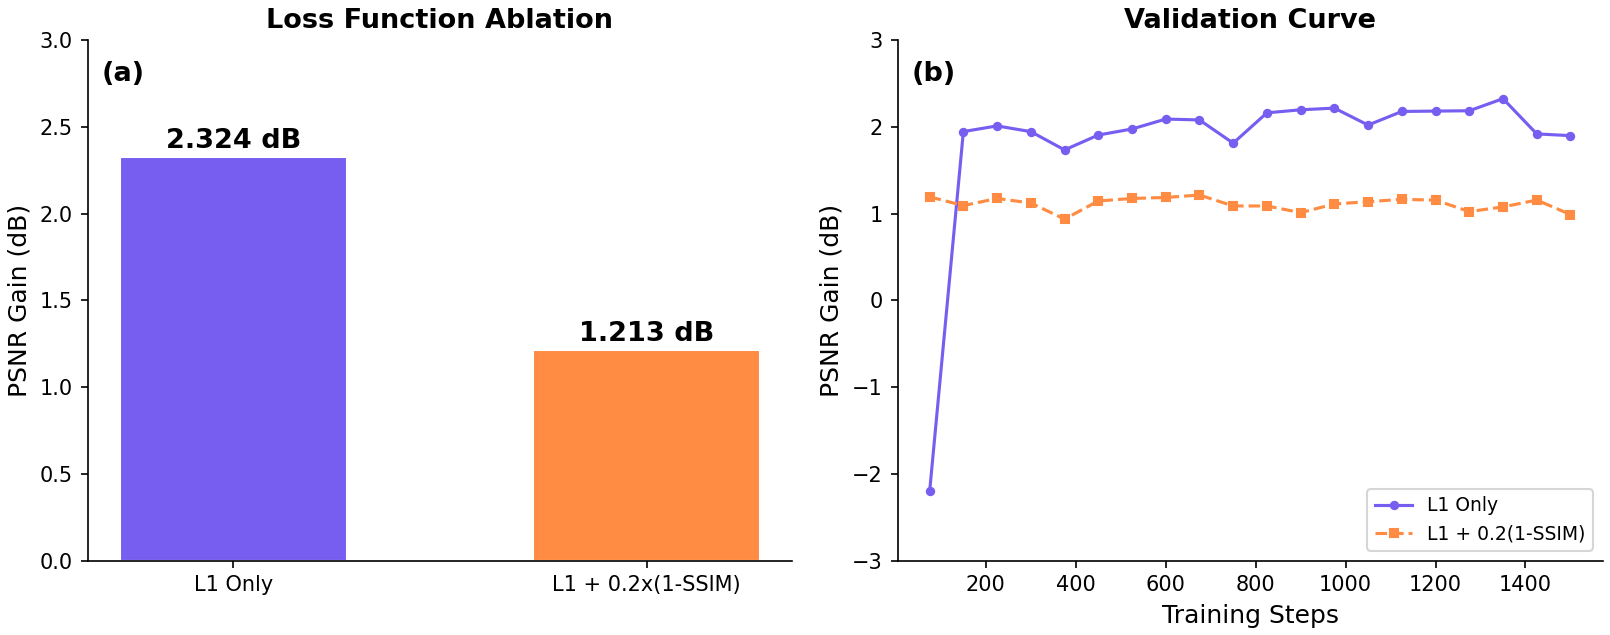
\includegraphics[width=0.92\textwidth]{loss_ablation.png}
  \caption{损失函数消融实验（a）PSNR Gain 对比（b）训练曲线}
  \label{fig:loss}
\end{figure}

该结果与直觉相反——通常认为结构一致性约束（SSIM）能提供结构先验从而辅助收敛，但在本任务中产生了显著的负面效应。需注意：SSIM 权重 0.2 为常用经验取值，本次消融仅验证该权重下的效果，不排除其他权重下复合损失存在提升空间。

现象的可能原因有三层。其一，SSIM 基于 $11\times11$ 滑窗内的局部均值和方差统计量，在 Rician 噪声主导的低信号区域，局部信号方差与噪声方差高度耦合，导致 SSIM 对真实结构退化和噪声波动的区分力不足，梯度偏向平滑噪声纹理而非恢复解剖边界。其二，本任务为严格配准的配对去噪场景，含噪图像与干净图像的解剖结构完全一致，仅存在像素级噪声扰动，不存在结构退化——SSIM 作为结构相似性指标，无法提供额外的结构先验引导，其梯度仅作用于噪声平滑，与 L1 的像素级去噪目标冗余甚至冲突。其三，也是这里差距较大的主要原因：复合损失中 L1 项采用 tissue-only 口径、SSIM 项采用全图口径，两者优化目标的空间范围不匹配，会在一定程度上加剧梯度冲突。但是在调整至现有口径之前，我已在全局统一口径下完成过同条件的 Stage A 消融实验，旧版结果图（见report\_figures\_old/loss\_ablation.png）显示纯 L1 损失的验证增益仍优于 L1+SSIM 复合损失，仅性能差距缩小至约 0.37 dB。这说明“纯 L1 更适配本任务”是稳健结论，不受口径选择的影响；当前采用分口径设置的原因（已在第~\ref{sec:metrics} 节（SSIM 全图计算的口径理由）和第~\ref{sec:protocol} 节（训练损失口径对齐）中说明，这里不再赘述。因此根据本阶段实验的结果可以认为，纯L1损失更适配本任务，后续实验全部采用纯 L1 损失。

### \subsection{Stage B：架构筛选}
5 类架构在 96 训练 $+$ 24 验证例、1500 步的同条件下对比（图~\ref{fig:arch}），结果呈极高密度的性能分布。

\begin{figure}[htbp]
  \centering
  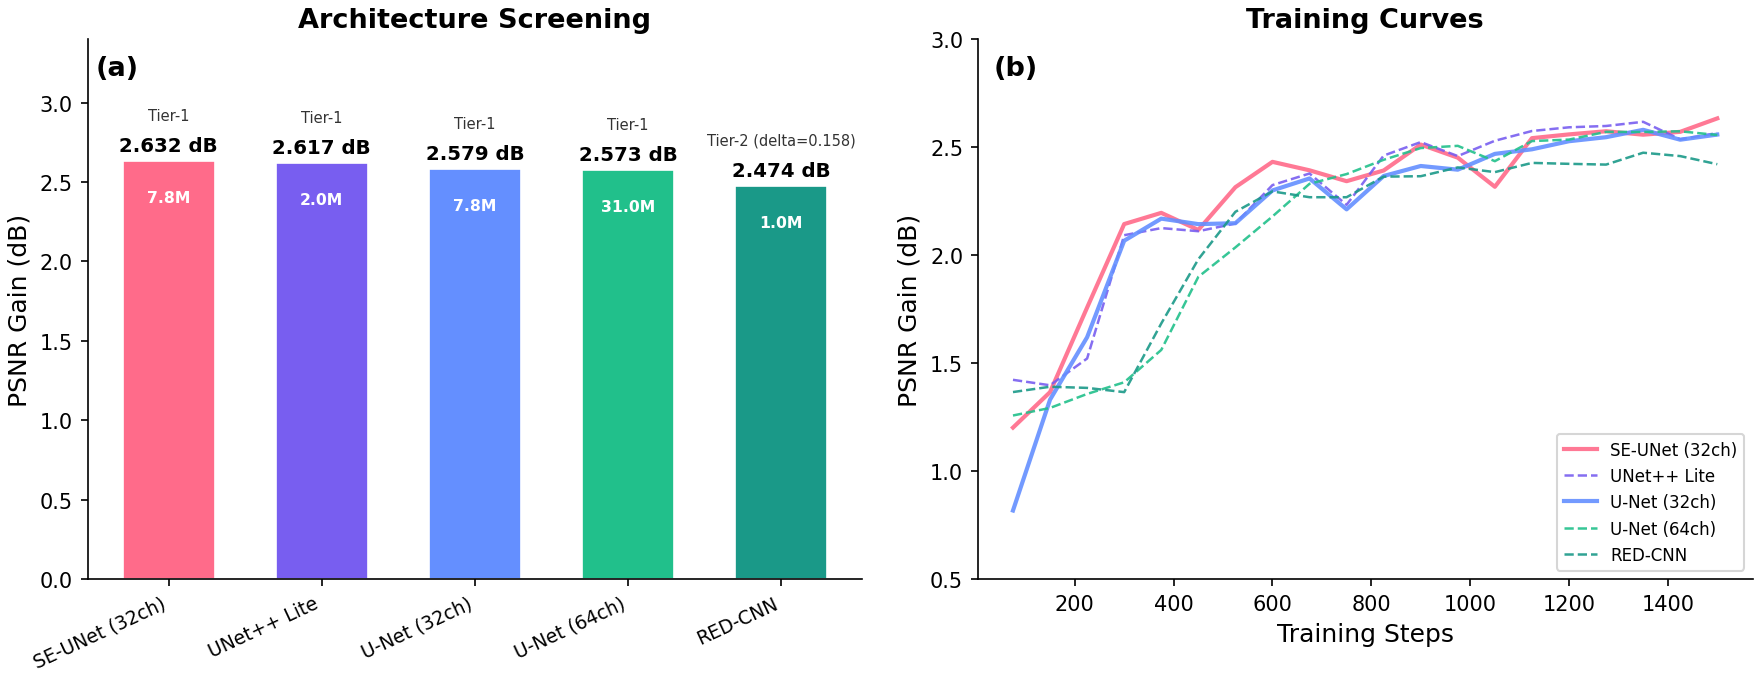
\includegraphics[width=0.95\textwidth]{arch_screening.png}
  \caption{架构筛选结果（120 例，1500 步）（a）PSNR Gain 对比（b）训练曲线}
  \label{fig:arch}
\end{figure}

图~\ref{fig:arch}a 显示：SE-UNet (32ch) 以 2.63\,dB 领跑，UNet++ Lite（2.62\,dB）、U-Net 32ch（2.58\,dB）、U-Net 64ch（2.57\,dB）紧咬其后，四者极差仅 0.06\,dB，均满足 Tier-1 标准（与第一名差距 $\le 0.1$\,dB）。RED-CNN 以 2.47\,dB 垫底，$\Delta=0.16$\,dB 超过 Tier-1 阈值，被划入 Tier-2，不进入 Stage C 和 Stage D。

就 SE 通道注意力的贡献而言，SE-UNet (32ch) 仅以 $+0.09$M 参数（$+1.1\%$）代价取得 0.05\,dB 的微弱领先。从任务特性看，T1 去噪以像素级噪声抑制为主，不涉及复杂语义类别区分，通道注意力可挖掘的增益空间本就有限，因此提升幅度微弱符合预期，说明 SE 注意力在 T1 去噪中存在可检测但幅度有限的正面贡献。

UNet++ Lite 的参数效率值得关注：以 2.00M 最少参数量（仅为 U-Net 32ch 的 25.7\%）达到 2.62\,dB 的次优性能。其嵌套密集跳连使浅层低阶特征可直接馈入解码器，训练早期就能快速拟合全局平滑结构；但该结构弱化了深层特征的语义聚合能力，对精细纹理的恢复后劲不足，因此训练中后期增速放缓，在 1500 步短步长下凭借收敛速度优势表现占优。

对比 U-Net 32ch 与 64ch，4 倍参数量差距仅换来 $-0.01$\,dB 的性能差异（几乎一致）。核心原因在于 $128\times128$ 单通道输入的特征维度有限，32 通道已足以覆盖 T1 脑影像的主要灰度模式与结构特征，通道翻倍带来的表征能力边际收益极低；加之固定步数下大模型单参数的梯度更新次数更少，进一步抵消了容量优势，说明在 1500 步预算下 32 个基础通道已提供足够的表示容量。

RED-CNN 性能较弱，本质源于架构设计的适配性不足：无池化的纯卷积堆栈不仅感受野增长缓慢，更缺少多尺度特征融合机制，无法同时兼顾局部噪声细节与全局噪声统计特性，因此在去噪任务中性能天然弱于 U 型编解码架构。

图~\ref{fig:arch}b 的训练曲线展示了收敛动态：SE-UNet 和 U-Net 32ch（实线）在 400 步后持续拉开与其余模型的差距，UNet++ Lite（虚线）训练初期领先但随后增速放缓。在 120 例、1500 步的预算下，全部 Tier-1 候选性能分布极窄，需要 Stage C 的跨种子重复实验提供额外判别信号。

本报告所有实验采用等步数比较，用于回答“相同训练预算下最优”的问题，而非各模型充分收敛后的理论上限。固定 epoch 会使大模型消耗更多算力，不适合资源受限场景。在本次总 GPU 时间约 2.3 小时的预算下，资源投入应视为建模成本的一部分；U-Net 64ch 在 1500 步下存在训练不充分而性能被低估的可能，若获得更多步数或可释放容量优势，但在目前预算下这一成本无法被忽略。

\subsection{Stage C：稳定性验证}
Stage C 对四种 Tier-1 模型进行中期训练（1000 步 $\times$ 3 种子）的独立重复（图~\ref{fig:stability}，表~\ref{tab:stability}）。

\begin{figure}[htbp]
  \centering
  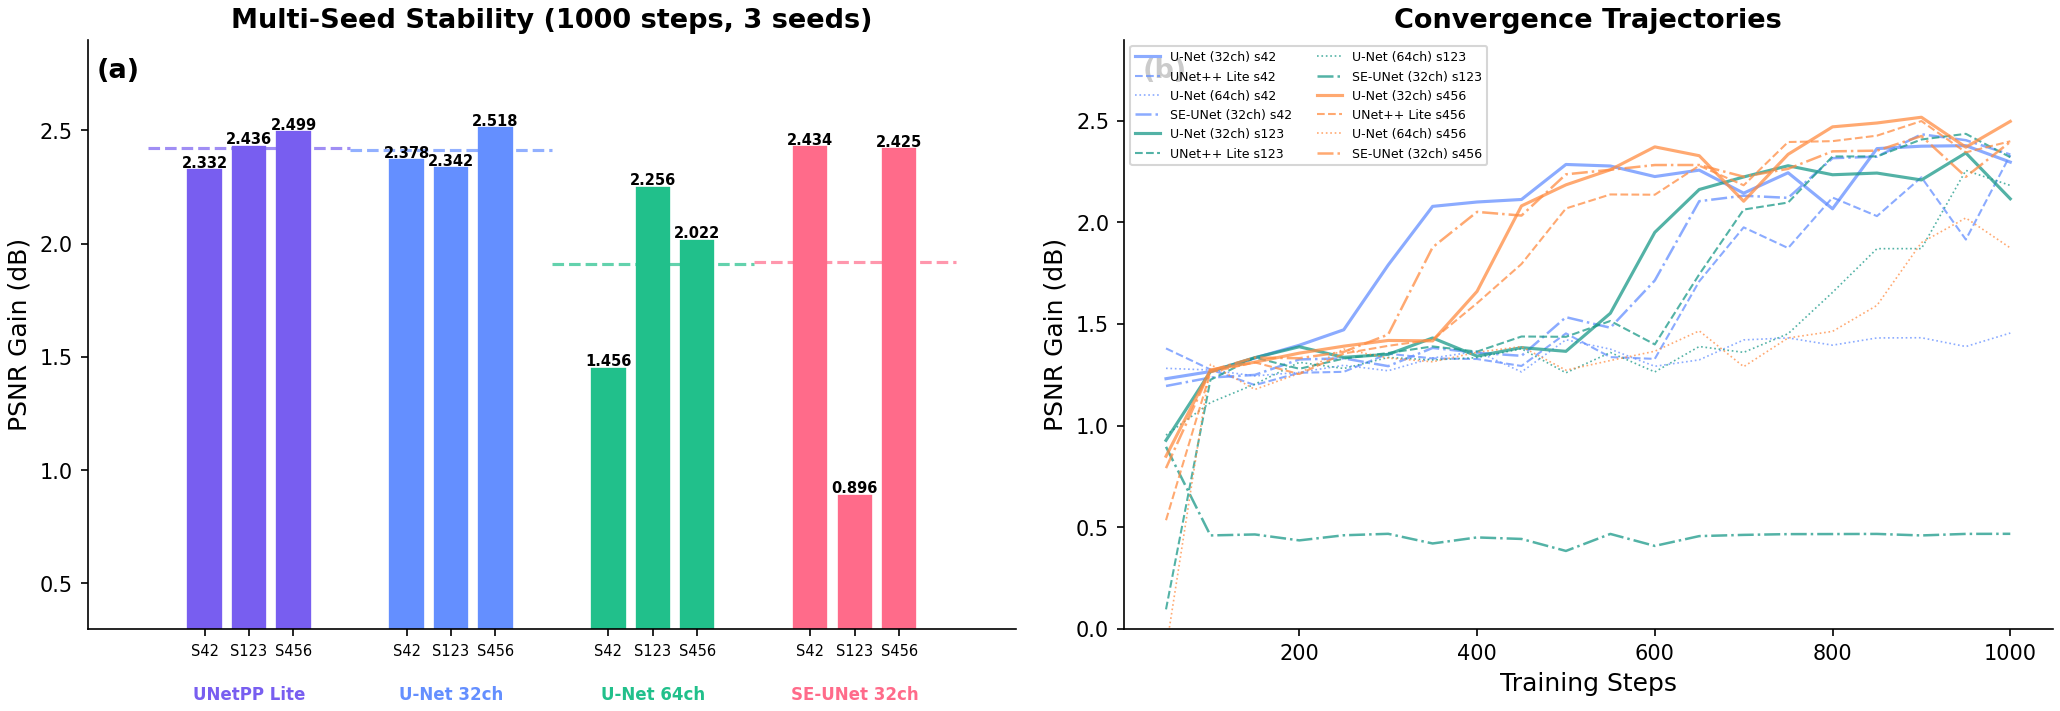
\includegraphics[width=0.95\textwidth]{multiseed_stability.png}
  \caption{跨种子稳定性验证（120 例，1000 步）（a）3 种子 PSNR Gain，虚线为均值（b）收敛轨迹}
  \label{fig:stability}
\end{figure}

\begin{table}[htbp]
  \centering
  \caption{Stage C 中期稳定性结果汇总（1000 步，3 种子，tissue-only 口径）}
  \label{tab:stability}
  \small
  \begin{tabular}{l c c c c c c}
    \toprule
    模型 & Seed 42 & Seed 123 & Seed 456 & Mean & Std & $2\sigma$ \\
    \midrule
    UNetPP Lite & 2.33 & 2.44 & 2.50 & 2.42 & 0.08 & 0.17 \\
    U-Net 32ch & 2.38 & 2.34 & 2.52 & 2.41 & 0.09 & 0.19 \\
    U-Net 64ch & 1.46 & 2.26 & 2.02 & 1.91 & 0.41 & 0.82 \\
    SE-UNet 32ch & 2.43 & \textbf{0.90} & 2.43 & 1.92 & 0.89 & \textbf{1.77} \\
    \bottomrule
  \end{tabular}
\end{table}

图~\ref{fig:stability} 和表~\ref{tab:stability} 共同揭示了三类跨种子行为模式（注意 Stage C 与 Stage B 的训练步数不同，均值绝对值不直接可比，稳定性分析聚焦于种子间离散度而非均值本身），其差异可从损失景观与架构特性层面得到解释：

第一类为高稳定性组，包括 UNet++ Lite 和 U-Net 32ch，两者跨种子标准差均 $\le 0.09$\,dB，$2\sigma$ 分别仅 0.17\,dB 和 0.19\,dB，图~\ref{fig:stability}b 中六条训练曲线紧密聚合，可复现性优秀。两者架构的损失曲面均较为平滑：UNet++ Lite 参数量少且梯度路径短，U-Net 32ch 参数量适中、无额外非线性门控，不同初始化下收敛终点差异小，因此跨种子一致性强。

第二类为中不稳定组——U-Net 64ch，跨种子 $2\sigma=0.82$\,dB，Seed 42 仅获 1.46\,dB 与 seed 123 的 2.26\,dB 相差 0.80\,dB。大参数量模型的损失景观更复杂，存在大量鞍点与局部极小值；1000 步训练不足以让模型遍历至全局最优区域，不同种子易停留在差异显著的局部最优点，因此波动幅度显著放大。

第三类为训练失效组——SE-UNet (32ch)，seed 123 下 val gain 仅 0.90\,dB，不到其他两个种子（2.43、2.43\,dB）的 40\%。其失效可能是因为SE 模块的 Sigmoid 门控若初始化落入饱和区，通道权重会持续接近 0，直接切断对应特征通路，导致编码器表征能力断崖式下降；且饱和区梯度近乎为零，短训练步数下无法依靠梯度累积脱离失效状态。该现象仅在 1000 步中期训练中观测到；5000 步全量训练下梯度的微小更新有可能逐步将门控拉出饱和区，因此不排除更长训练步数下失效种子可自行恢复。本次 3 种子观测中出现 1 例训练失效，提示该架构存在初始化敏感的收敛失败风险；实际使用时建议增加跨种子验证以规避此风险。

\subsection{Stage D：全量训练}
全量训练使用 480 训练 $+$ 60 验证 $+$ 60 测试，所有 Tier-1 模型统一跑满 5000 步。

\begin{figure}[htbp]
  \centering
  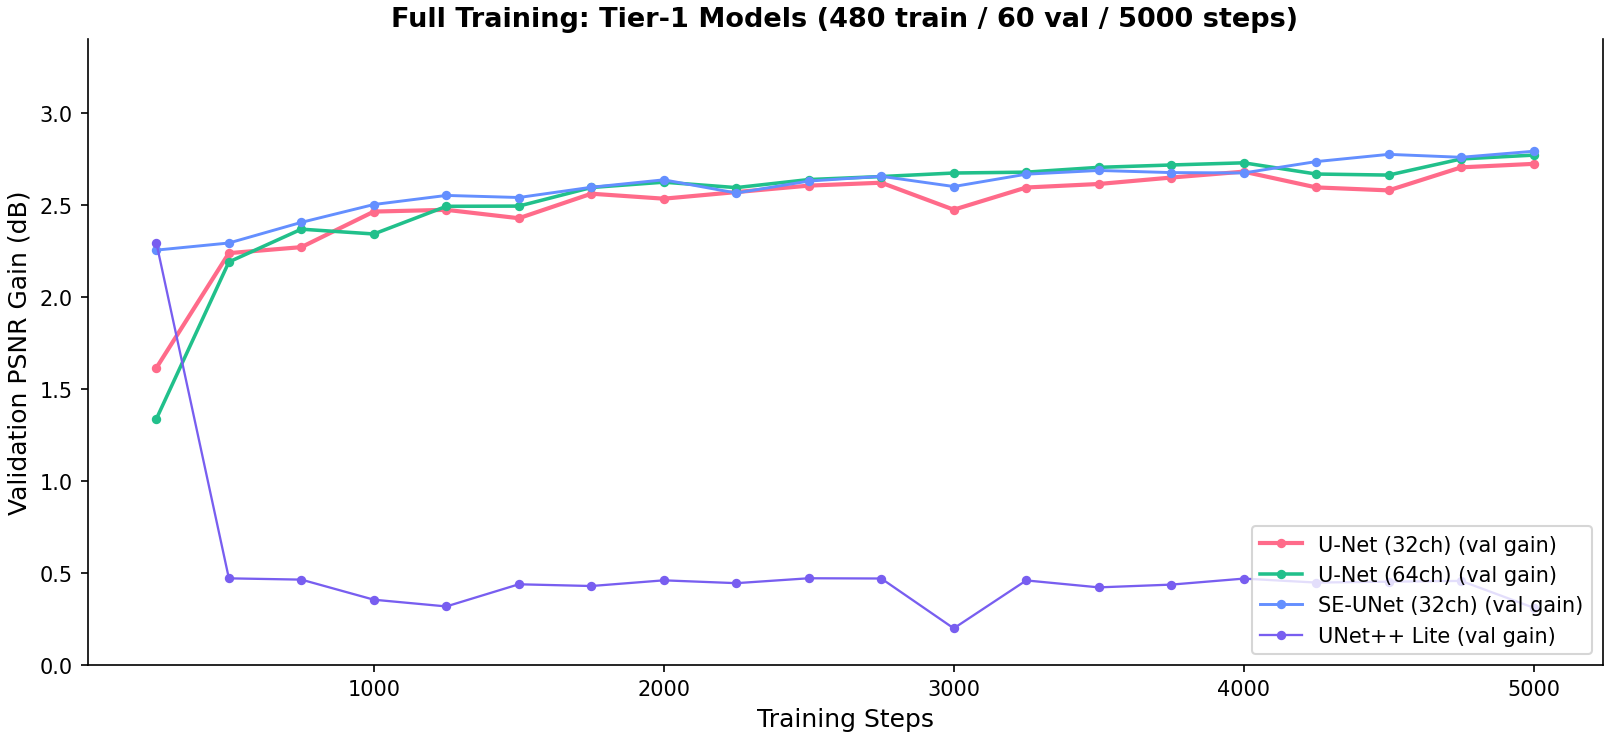
\includegraphics[width=0.95\textwidth]{full_train.png}
  \caption{全量训练验证曲线（480 训练例，5000 步），test 结果见表~\ref{tab:full}}
  \label{fig:full}
\end{figure}

图~\ref{fig:full} 展示 SE-UNet 和 U-Net 64ch 以相近速率交替领先，在约 3500 步后增速显著放缓；UNet++ Lite 的曲线从第一个评估点（step 250，增益 2.29\,dB）后便急剧下降并在约 0.3--0.5\,dB 的低位持续震荡，与其他三者持续上升的轨迹形成鲜明对比。3500 步后的增益趋缓是模型接近收敛的典型特征：此时大部分均匀组织区域的噪声已被充分压制，剩余优化空间仅集中于灰白质边界、脑沟等结构复杂的难例区域，误差下降的边际成本快速升高。

{\footnotesize\setlength{\tabcolsep}{4pt}
  \begin{longtable}{l r r r r r r l}
    \caption{Stage D 全量训练结果（5000 步，seed 42，tissue-only 口径）\label{tab:full}}\\
    \toprule
    模型 & Val Gain\textsuperscript{†} & Test Gain & Test PSNR & Test SSIM & Test MAE & Test ME & 参数量 \\
    \midrule
    \endfirsthead
    \toprule
    模型 & Val Gain\textsuperscript{†} & Test Gain & Test PSNR & Test SSIM & Test MAE & Test ME & 参数量 \\
    \midrule
    \endhead
    \bottomrule
    \endfoot
    SE-UNet (32ch) & 2.79 & 2.77 & 48.23 & 0.9959 & 0.00290 & $-3.1\!\times\!10^{-4}$ & 7.85M \\
    U-Net 64ch & 2.77 & 2.72 & 48.19 & 0.9956 & 0.00293 & $-7.4\!\times\!10^{-5}$ & 31.04M \\
    U-Net 32ch & 2.72 & 2.68 & 48.14 & 0.9954 & 0.00295 & $-5.8\!\times\!10^{-5}$ & 7.76M \\
    UNet++ Lite & 2.29 & 2.28 & 47.74 & 0.9923 & 0.00316 & $+1.1\!\times\!10^{-4}$ & 2.00M \\
    \bottomrule
    \multicolumn{8}{l}{\footnotesize † 所有模型均报告验证集最优 checkpoint（best.pt）的增益；UNet++ Lite 的最优 checkpoint 位于 step 250。}
  \end{longtable}}

结合表~\ref{tab:full} 多维度指标可进一步剖析各模型的性能差异与内在机制：

SE-UNet 以 test gain 2.77\,dB、test PSNR 48.23\,dB 稳居数值最优，相较 U-Net 32ch 的 0.09\,dB 优势虽幅度有限，但在 SSIM（0.9959 vs. 0.9954）、MAE（0.00290 vs. 0.00295）指标上保持了完全一致的排序，说明通道注意力带来的是像素精度与结构保真度的同步提升，而非单一指标的偶然波动。从 Stage B 到 Stage D，其相对 U-Net 32ch 的增益从 0.05\,dB 扩大至 0.09\,dB，印证了充足训练步数能逐步释放注意力模块的表征潜力——通道权重的精细校准需要更多迭代才能收敛至最优。

结合 Stage C 的观测，SE-UNet中期短训练下存在初始化敏感的收敛失效风险（$2\sigma=1.77$\,dB），根源是 Sigmoid 门控早期易落入饱和区导致梯度消失；而 5000 步全量训练下 seed 42 正常收敛，说明足够的梯度累积可逐步将门控拉出饱和区间，长训练能缓解但无法从根本上消除该风险，当然实际应用时仍需多种子验证兜底。

U-Net 32ch 是所有架构中综合均衡性最优的基准方案。精度层面，test gain 2.68\,dB、test PSNR 48.14\,dB 虽略低于 SE-UNet，但 0.09\,dB 的差距在单样本波动范围内，统计上不可分辨；SSIM 0.9954、MAE 0.00295 同样处于 Tier-1 模型的紧密区间内，结构保真度无实质短板。偏差校正层面，其 test ME 为 $-5.8\times10^{-5}$，是所有模型中绝对偏差最小的一档，说明 7.76M 的参数量与 L1 损失形成了极佳匹配——既充分校正了 Rician 正偏差，又未因模型容量过大引入额外的系统性低估。

更关键的是，其精度优势的代价极低：参数量仅为 U-Net 64ch 的 25\%，且 Stage C 中期跨种子波动仅 $2\sigma=0.19$\,dB，收敛稳定性远优于另外两种更大/更复杂的架构。这种“精度接近上限、稳定性拉满、参数量适中”的特性，使其成为资源受限场景下风险收益比最高的选择，也是本报告最终推荐方案的核心依据。

U-Net 64ch容量冗余，边际收益极低。4 倍参数量（31.04M vs. 7.76M）仅换来 test gain 提升 0.04\,dB、SSIM 提升 0.0002，且 ME 绝对值（$-7.4\times10^{-5}$）略小于 32ch 版本，说明通道数翻倍仅带来了极微弱的偏差校正与精度改善。本质原因在于 $128^2$ 分辨率的 T1 脑影像结构模式有限，32 个基础通道已足以覆盖灰白质、脑脊液等主要组织的灰度特征与空间分布，额外通道大多处于表征冗余状态。对应 Stage C 中其跨种子波动达 $2\sigma=0.82$\,dB，进一步印证大模型损失景观更复杂：短训练易停留在差异显著的局部最优点，长训练虽能收敛至相近精度，但参数量膨胀并未转化为对等的性能收益，参数效率显著偏低。

UNet++ Lite 呈现先升后崩的特殊收敛轨迹，并非简单欠拟合，而是小容量模型在大规模数据下的典型泛化坍塌。step 250 时模型仅接触约 6\% 的训练样本，能在有限病例上快速拟合出局部有效的去噪映射，形成短暂的性能峰值；随着更多解剖差异的样本输入，2M 参数不足以编码 480 例数据的分布多样性，梯度更新在不同样本的特征间反复拉扯，已学到的局部映射被持续覆盖，最终退化为仅能输出全局粗糙平滑的结果。

结合多指标可以发现，UNet++ Lite的test SSIM 仅 0.9923，与其余模型差距达 0.003 以上，说明结构保真度出现实质退化；test ME 为唯一正值（$+1.1\times10^{-4}$），表明模型已无力充分校正 Rician 正偏差，残留了原始噪声的偏差特性。该现象也反向解释了 Stage B 中小样本下其性能靠前的原因——短步长+小数据的场景中，收敛速度优势掩盖了容量上限的短板，只有全量训练才能暴露模型的真实适配边界。

四类模型的 SSIM 处于 0.9923--0.9959 的极窄区间，极差仅 0.0036，说明当前任务下结构相似性先于像素精度触及性能天花板，后续优化更多集中于像素级误差的精细校正，而非结构层面的改善。MAE 排序与 PSNR 完全一致，验证了误差幅度度量的自洽性；ME 的符号与量级则与模型去噪能力正相关——性能越强的模型，ME 越接近零且呈现 L1 损失特有的微弱负偏，从偏差校正维度进一步佐证了性能排序的可靠性。

\subsection{最终推荐方案}

\begin{figure}[htbp]
  \centering
  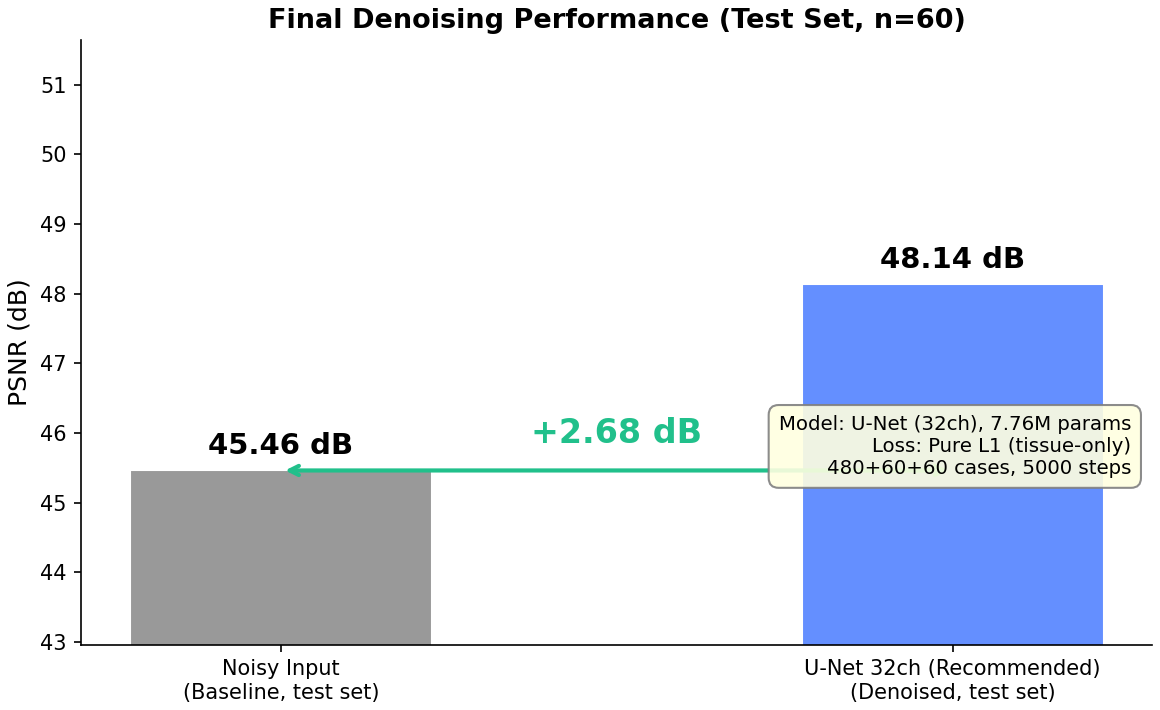
\includegraphics[width=0.75\textwidth]{final_result.png}
  \caption{U-Net 32ch（推荐方案）在独立测试集（n=60）上的去噪性能}
  \label{fig:final}
\end{figure}

综合全部四阶段实验证据（图~\ref{fig:final}，表~\ref{tab:full}）：

\begin{itemize}
  \item SE-UNet (32ch) 在 seed 42 下精度最优（48.23\,dB，较噪声图像提升2.77\,dB），但 Stage C 中期观测到 seed 123 训练失效（$2\sigma=1.77$\,dB），存在初始化敏感的收敛失败风险。
  \item U-Net 64ch 以 4 倍于U-Net 32ch参数量精度却仅进一步提升 $+0.05$\,dB ，参数效率极低，跨种子波动亦非最优（$2\sigma=0.82$\,dB）。
  \item UNet++ Lite 全量数据下出现容量$-$数据错配——验证增益从 step 250 的 2.29\,dB 崩溃至训练终点 0.3--0.5\,dB，2M 参数容量无法适配 480 例数据规模。
  \item U-Net 32ch 在所有维度均衡——精度仅落后最优SE-UNet (32ch) 0.09\,dB（几乎一致），中期训练跨种子 $2\sigma=0.19$\,dB（可复现性优异），7.76M 参数适中。
\end{itemize}

综合以上证据，本报告推荐 U-Net 32ch 为最终方案。选型依据是跨种子稳定性与可复现性——Tier-1 候选间精度极度接近，而稳定性维度提供了关键的区分信号。跨种子稳定性直接决定实验的可复现性与工程落地成本：U-Net 32ch 的低波动（$2\sigma=0.19$\,dB）意味着单次训练即可获得稳定可靠的结果，无需多次重复筛选最优种子，在资源受限的科研场景与批量部署中具有更高的实用价值。稳定性结论基于 Stage C 中期训练（1000 步）观测，全量收敛后的长期稳定性仍待进一步验证。

\subsection{病例可视化与定性分析}

\begin{figure}[htbp]
  \centering
  \begin{subfigure}{0.48\textwidth}
    \centering
    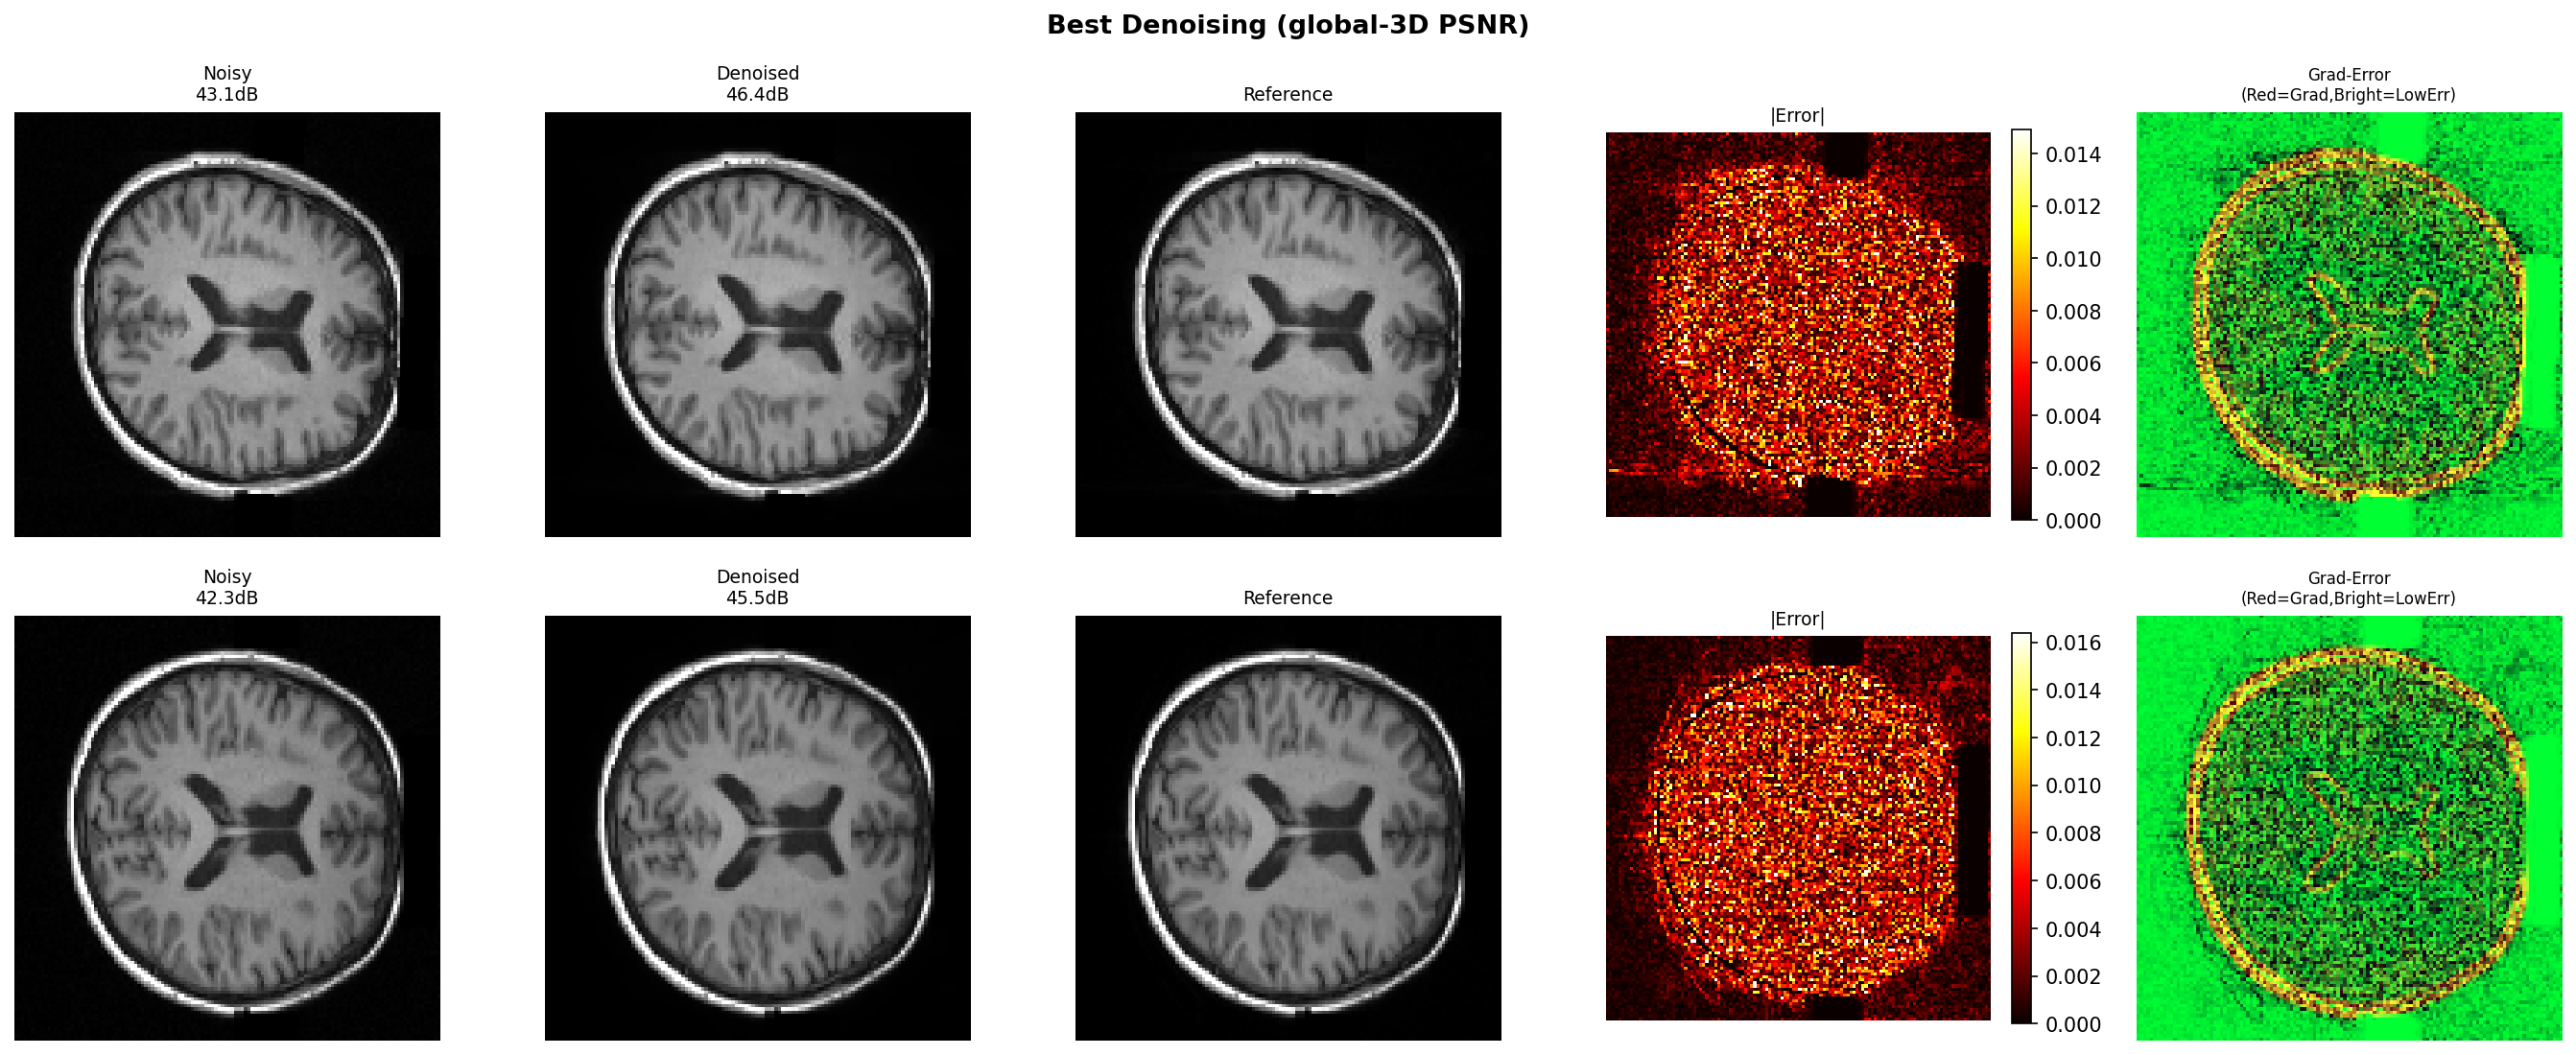
\includegraphics[width=\textwidth]{triplet_best.png}
    \caption{最佳增益病例}
    \label{fig:triplet_best}
  \end{subfigure}
  \hfill
  \begin{subfigure}{0.48\textwidth}
    \centering
    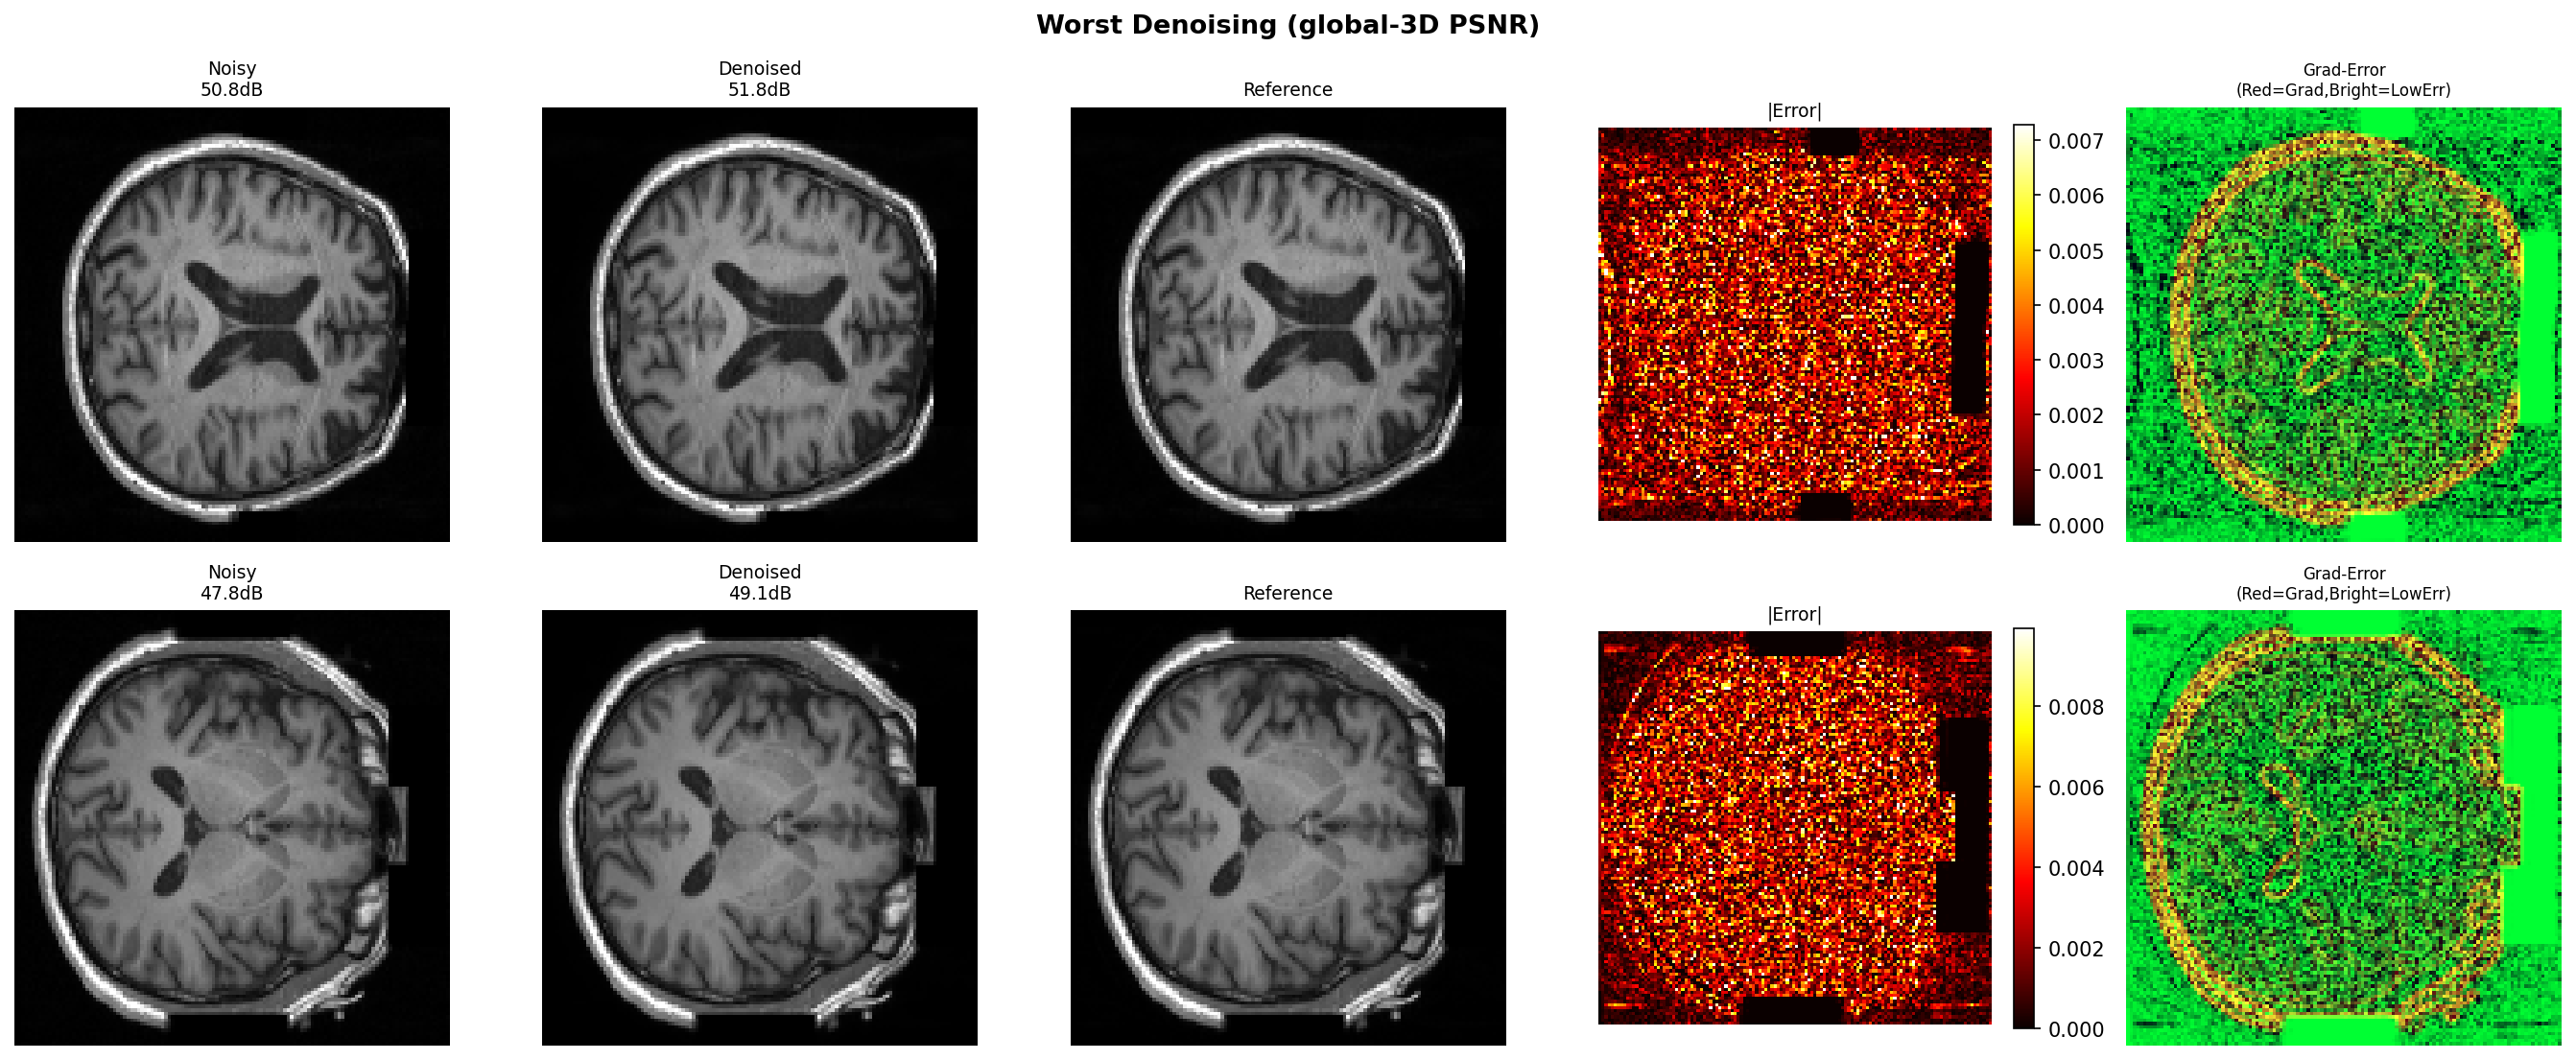
\includegraphics[width=\textwidth]{triplet_worst.png}
    \caption{最低增益病例}
    \label{fig:triplet_worst}
  \end{subfigure}
  
  \vspace{0.3cm}
  \begin{subfigure}{0.48\textwidth}
    \centering
    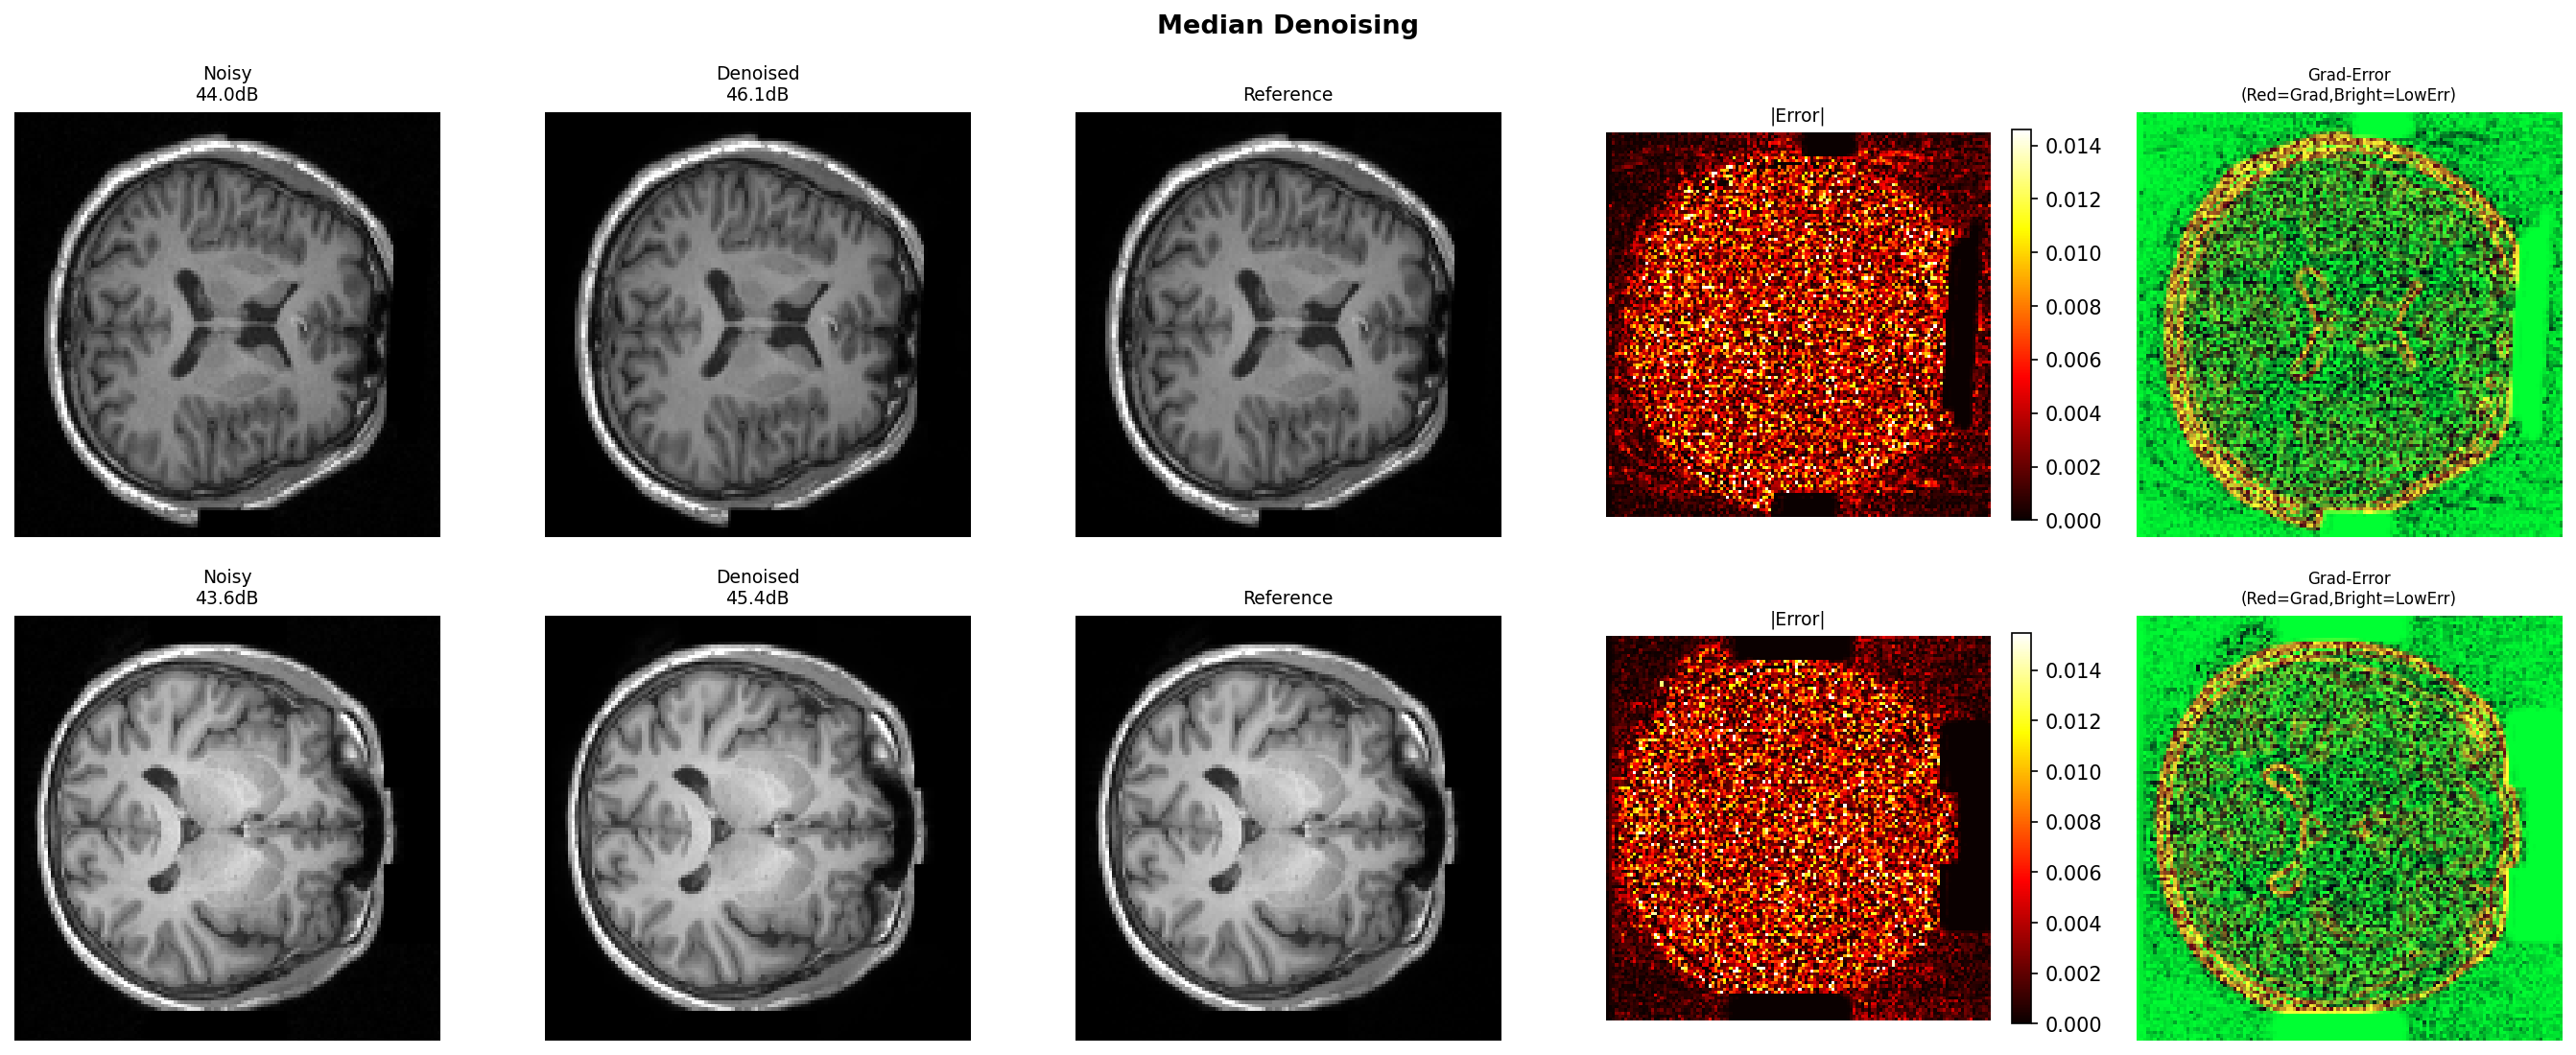
\includegraphics[width=\textwidth]{triplet_median.png}
    \caption{中位增益病例}
    \label{fig:triplet_median}
  \end{subfigure}
  \caption{测试集定性可视化（U-Net 32ch）（a）最佳增益（b）最低增益（c）中位增益病例}
  \label{fig:triplets}
\end{figure}

以 U-Net 32ch 对测试集 60 例进行推理，提取增益最高、最低及中位病例进行定性可视化（图~\ref{fig:triplets}）。每幅子图自上而下三行：含噪输入、去噪输出与干净参考的原始图像，三者局部放大细节（聚焦灰白质交界或脑沟/脑回结构），以及去噪误差图、梯度$-$误差联合图（梯度模 $>$ 阈值品红着色）和含噪误差图；所有误差图使用统一的 $[-0.08, 0.08]$ 色彩映射范围。

最佳增益病例（图~\ref{fig:triplet_best}）：该病例（3D gain $\approx$ 3.90\,dB）初始含噪图像中灰白质边界和皮层沟回处存在明显的结构模糊。去噪后这些高对比度解剖边界得到清晰恢复，局部放大细节中去噪输出与干净参考的差异肉眼难辨。该病例噪声水平较高，低信号的脑沟、灰白质边界处Rician正偏差尤为显著，恰好对应模型去噪增益最显著的区间，与信号分箱中“低信号区增益最高”的结论完全吻合。绝对误差图显示误差几乎全部集中在解剖边界和脑沟区域；梯度$-$误差联合图进一步揭示误差具有强梯度依赖性：图像梯度大的结构突变处对应误差峰值，梯度近乎为零的白质均匀区误差接近零，说明模型残留误差全部来自结构与噪声的混叠区域，均匀组织内已实现近乎无偏恢复，未引入额外平滑伪影。

最低增益病例（图~\ref{fig:triplet_worst}）：该病例（3D gain $\approx$ 0.77\,dB）的初始含噪图像 PSNR 极高（$\approx$ 50.31\,dB），含噪图在视觉上与干净参考几乎无异。这不是模型失效，而是度量天花板效应：该病例本底信噪比极高，噪声幅值小导致Rician正偏差本身微弱，模型的可优化空间被天然压缩。对比最佳病例可见，其绝对误差色阶上限仅约为最佳病例的一半，残留误差的绝对幅值本就很低；增益数值小更多反映了PSNR指标在高信噪比区间的灵敏度下降，而非去噪效果差。该病例的存在也说明数据集内噪声水平的病例间差异显著（标准差比例范围 0.013--0.042）。

中位病例（图~\ref{fig:triplet_median}）：误差模式同样集中于灰白质交界和皮层沟回处，深部白质核心和脑室附近误差极低——与 T1 的组织信号分布一致。其误差分布模式与最佳病例高度一致，说明模型的误差规律具有跨病例的稳定性，泛化表现可靠。所有去噪输出均未引入可见的结构伪影，残差学习在压制噪声的同时完整保留了皮层褶皱与灰白质边界的纹理细节，未出现过平滑现象，适配后续脑影像分割、配准等分析任务的需求，纹理保真度优势明显。

\subsection{Rician 信号依赖性的实证验证}
按脑组织掩膜内干净图强度将全部 6602 个有效切片三等分，所有 PSNR/ME 口径与主表一致（tissue-only）。图~\ref{fig:signalbin} 以柱高表示各分区 PSNR Gain，红色/蓝色标注分别对应含噪 ME 和预测 ME 的方向及量级。

\begin{figure}[ht]
  \centering
  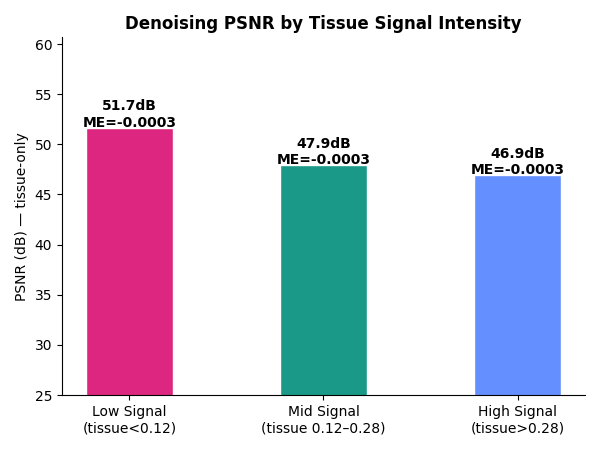
\includegraphics[width=0.75\textwidth]{signal_bin_bar.png}
  \caption{信号强度分箱分析（tissue-only 口径），定量结果见表~\ref{tab:signalbin}}
  \label{fig:signalbin}
\end{figure}

\begin{table}[ht]
  \centering
  \caption{脑组织内信号分箱定量结果（tissue-only 口径，U-Net 32ch 输出）}
  \label{tab:signalbin}
  \small
  \begin{tabularx}{\linewidth}{l c c r r r r}
    \toprule
    信号区间 & 切片数 & 组织均值 & PSNR & Gain & Pred ME & Noisy ME \\
    \midrule
    低信号（CSF/边缘） & 803 & [0.01, 0.12) & 51.67 & 6.72 & $-3.4\!\times\!10^{-4}$ & $+3.5\!\times\!10^{-3}$ \\
    中信号（灰质）& 4765 & [0.12, 0.28) & 47.94 & 2.36 & $-3.1\!\times\!10^{-4}$ & $+1.6\!\times\!10^{-3}$ \\
    高信号（白质）& 1034 & [0.28, 0.38] & 46.92 & 1.58 & $-3.3\!\times\!10^{-4}$ & $+1.2\!\times\!10^{-3}$ \\
    \bottomrule
  \end{tabularx}
\end{table}

图~\ref{fig:signalbin} 和表~\ref{tab:signalbin} 从噪声统计、偏差校正、损失特性三个层面，为 Rician 噪声的信号依赖性提供了闭环实证。

去噪增益随信号强度呈严格单调递减：低信号区增益 6.72\,dB，分别为中、高信号区的 2.8 倍和 4.3 倍。这一梯度完全契合 Rician 分布的数学本质——幅度图像的噪声方差随信号幅值降低而升高，低信号区本底噪声更大，可优化空间更充足，因此增益更高。占切片总量 72\% 的中信号区增益为 2.36\,dB，是全局去噪性能的核心贡献来源；分箱加权均值与全局 test gain（2.68\,dB）仅相差约 0.1\,dB，差异源于分箱边界的切片归属，整体趋势自洽。

含噪 ME 的梯度进一步验证了 Rician 正偏差的信号依赖性：从低信号区的 $+3.5\times 10^{-3}$ 到高信号区的 $+1.2\times 10^{-3}$，偏差幅度随信号升高单调下降，与 Rician 分布“右偏程度随信噪比降低而加剧”的特性完全对应。

去噪后三个区间的 Pred ME 高度一致，均稳定在 $-3\times 10^{-4}$ 量级，较原始偏差压缩约 7 倍，且符号统一为负。这说明两点：其一，通用 L1 残差学习无需针对 Rician 做专项设计，即可均匀校正不同信号强度下的正偏差，没有出现低信号区校正不足、高信号区过校正的分化；其二，残留的微弱负偏差是 L1 损失的固有统计属性——L1 优化目标是条件中位数，而右偏的 Rician 分布中位数天然低于均值，因此输出会系统性轻微低估，该偏差量级极小，对后续影像分析无实质影响。

低信号区的超高增益需审慎解读。该区域仅占总切片的 12\%，且信号幅值极低，噪声波动可接近甚至超过信号本身。受 PSNR 的对数计算特性影响，基线 MSE 越高，相同绝对误差下降带来的 dB 增益就越大；6.72\,dB 的增益更多反映了基线信噪比极低的数学效应，并不等价于该区域解剖结构的恢复程度优于高信号区。

这一特性也可直接解释 Stage A 中复合损失的失效：低信号区是去噪增益的主要来源，但该区域噪声与精细结构高度混叠，SSIM 基于局部窗口的统计量无法区分噪声波动与真实解剖边界，无法提供有效梯度引导，反而拖慢整体收敛。

综上，增益梯度匹配 Rician 方差-信号关系、含噪 ME 追踪 Rician 正偏差分布、去噪后 ME 验证偏差校正效果，共同证实通用 L1 残差学习已能有效压制 Rician 正偏差的主体成分。需说明的是，ME 为区域均值指标，无法刻画组织内部更细粒度的偏差异质性。

\subsection{参数效率权衡}

\begin{figure}[ht]
  \centering
  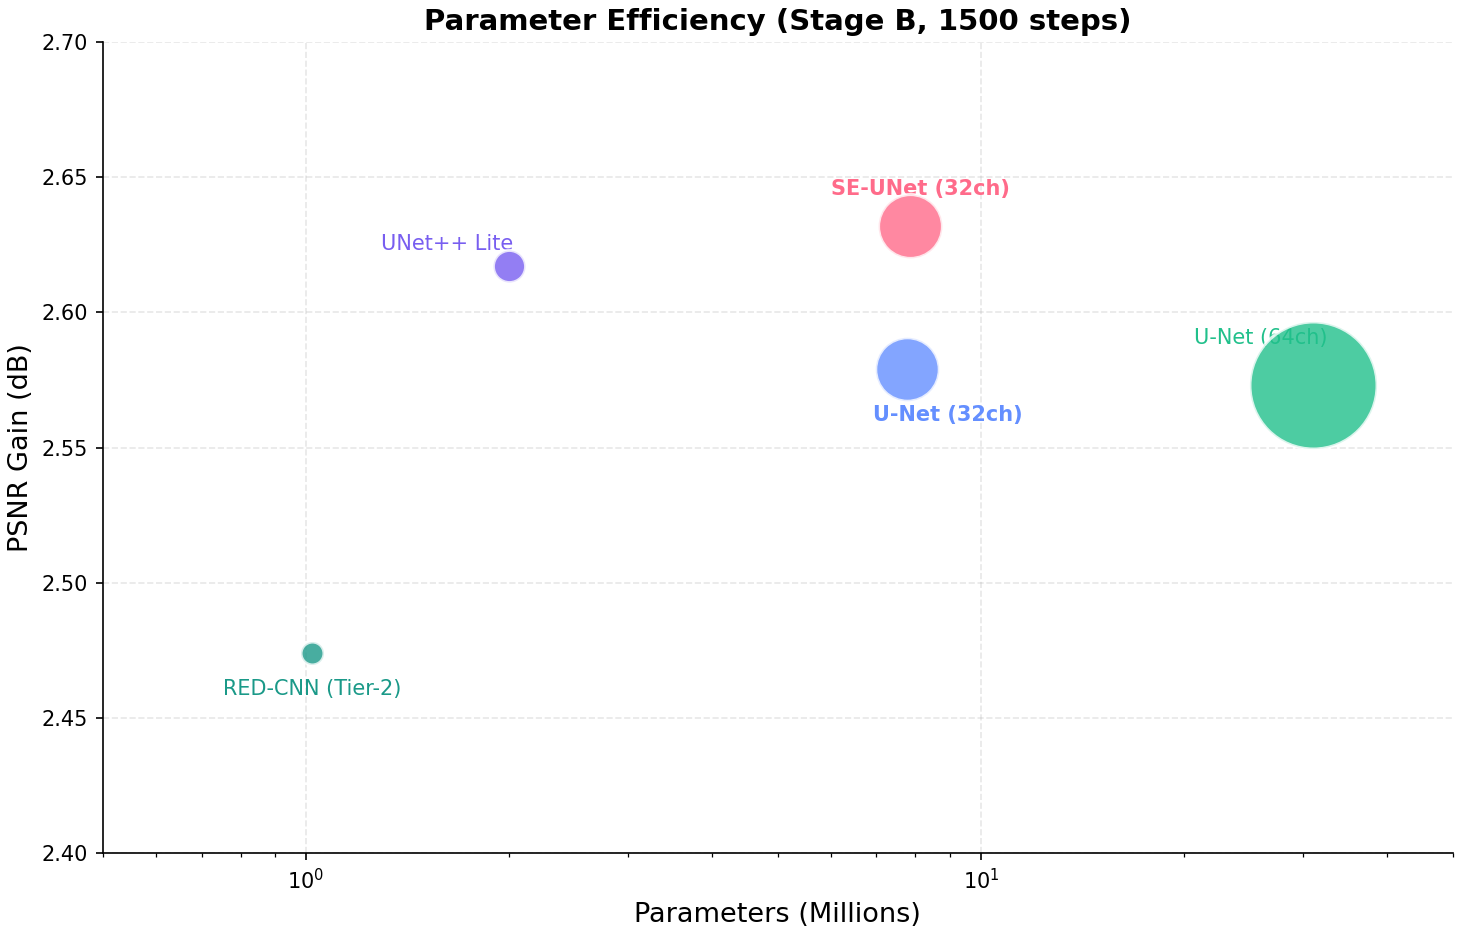
\includegraphics[width=0.78\textwidth]{param_efficiency.png}
  \caption{参数—性能权衡（Stage B，1500 步）}
  \label{fig:param}
\end{figure}

图~\ref{fig:param} 将 Stage B 中五种架构的参数—性能权衡可视化，图中各模型的气泡大小反映了模型参数量的大小。该图揭示了几条不同的设计路径。

极限参数效率路径以 UNet++ Lite 为代表：2.00M 参数在 Stage B 达到 2.62\,dB，单位参数增益 1.31\,dB/M，是 U-Net 32ch（0.33\,dB/M）的 4.0 倍。但其全量训练中性能崩溃至 0.3--0.5\,dB（最终 test gain 2.28\,dB 来自早期 snapshot，不代表稳定收敛），表明极稀疏参数化下性能与数据规模的良性扩展存在硬上限。

UNet++ Lite 的参数效率也印证了效率的场景依赖性：小样本阶段其极高参数效率本质是短梯度路径带来的收敛速度优势 $+$ 容量与 120 例数据的匹配；当数据量与训练步数同时扩展至 480 例 $\times$ 5000 步，收敛速度红利消失、容量短板暴露，参数效率优势便不复存在。

稳健均衡路径以 U-Net 32ch 为代表：7.76M 参数，跨阶段表现最一致——Stage B 2.58\,dB、Stage C $\mu=2.41$\,dB、Stage D 2.68\,dB。其参数—性能—稳定性三角均衡是当选最终推荐方案的根本原因。

容量浪费路径以 U-Net 64ch 为代表：31.04M 参数（$\times 4$），Stage B gain 仅 2.57\,dB（$-0.01$\,dB vs.\ 32ch）。在固定步数预算下，超大参数量使每个参数获得更少的梯度更新，等效于训练不充分。

注意力增强路径以 SE-UNet (32ch) 为代表：以仅 $+1.1\%$ 参数增量（$+0.09$M）取得 $+0.05$\,dB 增益（相比不加注意力的U-Net 32ch）。该路径挑战不在参数量，而在稳定性。

RED-CNN（1.02M，2.47\,dB）参数最少但增益也最低，说明其 5 层对称 $3\times 3$ 卷积堆栈的表示效率低于 U-Net 系列的编码器$-$解码器架构。

\subsection{局限与展望}
本文存在若干局限值得后续改进。首先，当前采用 2D 切片逐层处理，未利用 z 轴层间连续性，改用 3D 卷积或 2.5D 多切片输入预期可获额外增益~\cite{Zhao2021MC3DCNN}。其次，结论仅基于 T1 加权与单次数据划分（80/10/10, seed 42），泛化性仍有待交叉验证确认。在稳定性评估方面，Stage C 受算力资源限制，仅覆盖 3 个种子，扩大至 $\ge 10$ 个种子的扫描将提供更可靠的稳定性估计；同时跨种子稳定性结论基于 1000 步中期观测，全量 5000 步下的长期波动仍需进一步验证。此外，信号分箱使用了简单的三等分划分，若引入组织类别特异性分析（如经 FSL FAST 分割为 CSF、灰质、白质）可提供更精细的组织级见解。

\section{结论}
本报告通过``三层递进评估 $+$ 一层全量验证''的框架，对 UK Biobank T1 脑 MRI 去噪任务进行了系统的训练配置遴选。

在损失函数层面，纯 L1 损失（tissue-only 口径）以 val gain 2.32\,dB 显著优于 L1$+$SSIM 组合（1.21\,dB），Rician 噪声下 SSIM 的信号$-$噪声区分力不足、结构先验冗余以及优化空间不匹配共同导致复合损失失效。

在架构层面，五类候选经三层递进筛选后的最终结果为：SE-UNet 以 test PSNR 48.23\,dB（gain 2.77\,dB）取得数值最优，但中期跨种子观测暴露出 1 例训练失效（$2\sigma=1.77$\,dB），SE 通道注意力以 $+1.1\%$ 参数增量换取 $+0.09$\,dB 增益的代价是收敛敏感风险；UNet++ Lite 以 2.00M 最少参数量在 Stage B 取得 2.62\,dB，但在全量 480 例 $\times$ 5000 步下因容量$-$数据错配发生泛化坍塌，验证增益从 step 250 的 2.29\,dB 崩溃至训练终点 0.3--0.5\,dB，揭示了筛选阶段小样本高估偏差与容量上限的双重约束。综合权衡后，U-Net 32ch 以 test PSNR 48.14\,dB（gain 2.68\,dB）和 mid-training 跨种子 $2\sigma=0.19$\,dB 实现精度和稳定性的最优折衷，较 NLM 传统基线（gain 0.81\,dB）提升 3.3 倍。

信号分箱与 ME 追踪进一步揭示 Rician 噪声的信号依赖性——增益梯度从低信号区的 6.72\,dB 递减至高信号区的 1.58\,dB，去噪后 ME 全局收束至 $-3.1\times 10^{-4}$，证实通用 L1 残差学习已能有效压制 Rician 正偏差的主体成分。

全文实验基于 Ubuntu 22.04 + CUDA 12.8.1 + PyTorch 2.10 环境，``三层递进评估''框架以总 GPU 时间约 2.3 小时完成一次完整闭环，实验日志、中间结果和最终输出均可通过固定种子与预置脚本完整复现。

\bibliographystyle{plain}
\bibliography{references}

\section*{附录}

\subsection*{A\quad 代码与实验复现}

本项目 GitHub 仓库地址：\url{https://github.com/daomuyang/CNPJ_Liesen_Gai}。仓库已上传全部代码、预处理脚本、报告源文件（\texttt{report.tex}/\texttt{report.pdf}）、图表（\texttt{report\_figures/}）及 \texttt{README.md}；\texttt{.DS\_Store}、\texttt{\_\_pycache\_\_/}、LaTeX 编译临时文件等未上传。完整项目结构见仓库中的 \texttt{README.md}。

\subsection*{B\quad 实验环境与复现步骤}

实验环境：Ubuntu 22.04，CUDA 12.8.1，Python 3.12.13，PyTorch 2.10.0，GPU NVIDIA A10（24 GB）。

完整复现流程：

\begin{enumerate}
  \item 克隆仓库并配置环境：
  \begin{verbatim}
  git clone https://github.com/daomuyang/CNPJ_Liesen_Gai.git
  cd CNPJ_Liesen_Gai/CNPJ/
  python3 -m venv .venv && source .venv/bin/activate
  pip install -r requirements.txt
  \end{verbatim}

  \item 准备数据：将 UK Biobank T1 数据集复制至 \texttt{data/raw/} 目录下，每例一个子文件夹，内含 \texttt{T1\_noisy.nii.gz} 和 \texttt{T1\_clean.nii.gz}。目录结构为\\ \texttt{data/raw/\{caseid\}/T1\_noisy.nii.gz} 与 \texttt{data/raw/\{caseid\}/T1\_clean.nii.gz}。

  \item 下载所有实验结果：从百度网盘（链接见下文）下载 \texttt{experiments/} 文件夹，解压后放置于 \texttt{CNPJ/experiments/}。
  
  {\small\raggedright 百度网盘：\url{https://pan.baidu.com/s/1mEfSFJ5ys1GsNMqpV41tRQ?pwd=2xx2}\quad 提取码：\texttt{2xx2}\par}

  \item 按序运行实验：
  \begin{verbatim}
  python preprocess.py          # 预处理（生成 data/preprocessed/）
  python run_preliminary.py     # 预实验 Stage A+B+C（约 83 分钟）
  python run_full_train.py      # 全量训练 Stage D（约 54 分钟）
  python run_baseline.py        # NLM 传统基线（可选，约 30 分钟）
  python run_visualization.py   # 后处理可视化（约 3 分钟）
  python generate_figures.py    # 生成报告图表
  \end{verbatim}

  \item 编译报告：
  \begin{verbatim}
  xelatex report.tex && xelatex report.tex
  \end{verbatim}
\end{enumerate}

\subsection*{C\quad 模型选择建议}

本报告基于“三层递进评估 $+$ 一层全量验证”框架，对五类架构进行了系统筛选。根据不同使用场景，给出以下模型选择建议：

\begin{itemize}
  \item \textbf{精度$-$稳定性综合最优（推荐方案）：U-Net 32ch。}test PSNR 48.14\,dB（增益 2.68\,dB），跨种子 $2\sigma=0.19$\,dB，7.76M 参数适中。单次训练即可获得稳定可靠结果，适合科研复现与批量部署。

  \item \textbf{纯精度最优（需额外验证种子稳定性）：SE-UNet 32ch。}test PSNR 48.23\,dB（增益 2.77\,dB），以仅 $+1.1\%$ 参数增量换取 $+0.09$\,dB 提升。3 次种子观测中出现 1 例训练失效（$2\sigma=1.77$\,dB），建议至少运行 5--10 次独立种子训练，选取验证集最优 checkpoint 以避免收敛失败。适合可在充足算力下进行跨种子验证的场景。

  \item \textbf{参数效率最优（小样本/短训练场景）：UNet++ Lite。}2.00M 参数在 120 例 1500 步下达到 2.62\,dB 增益，单位参数效率为 U-Net 32ch 的 4 倍。嵌套密集跳连提供短梯度路径，在小数据和短步长下收敛极快。但全量 480 例 5000 步下因容量不足出现泛化坍塌——仅适用于训练数据量不超过 $\sim$120 例的有限预算场景，不适配大数据量全量训练。

  \item \textbf{高容量方案（不推荐，性价比极低）：U-Net 64ch。}31.04M 参数（4 倍于 32ch），test gain 2.72\,dB 仅高出 $+0.05$\,dB，跨种子 $2\sigma=0.82$\,dB。在 $128^2$ 分辨率下，32 基础通道已触及 U-Net 架构的表示容量上限，翻倍通道数无法带来实质增益。

  \item \textbf{最低参数量方案（不推荐，性能上限低）：RED-CNN。}1.02M 参数，Stage B gain 2.47\,dB（$\Delta=0.16$\,dB vs. 最优），因感受野线性增长限制全局噪声建模能力，未进入后续筛选。
\end{itemize}

\end{document}
